\documentclass[11pt,handout,aspectratio=169]{beamer}


%%%%%%%%% GENERAL PACKAGES
%\usepackage{xcolor}
%\usepackage{pdfpages}
%\usetheme[progressbar=frametitle]{metropolis}
%\setbeamercolor{background canvas}{bg=white}
%\usepackage{appendixnumberbeamer}
%\usepackage{booktabs}
%\usepackage[scale=2]{ccicons}
%\usepackage{pgfplots}
%\usepgfplotslibrary{dateplot}
%\usepackage{xspace}
%\newcommand{\themename}{\textbf{\textsc{metropolis}}\xspace}
%\usepackage[absolute,overlay]{textpos}

%%%%%%%%% COLOR THEME

% Define some colors:
\definecolor{DarkFern}{HTML}{407428}
\definecolor{DarkCharcoal}{HTML}{4D4944}
\definecolor{AlertColor}{RGB}{89,124,158}
\definecolor{HighLight}{RGB}{96,95,134}
\definecolor{Important}{RGB}{234,122,133}
\definecolor{Yellow}{HTML}{00539C}
\colorlet{Fern}{DarkFern!85!white}
\colorlet{Charcoal}{DarkCharcoal!85!white}
\colorlet{LightCharcoal}{Charcoal!50!white}
\colorlet{HighLight2}{AlertColor}
\colorlet{DarkRed}{red!70!black}
\colorlet{DarkBlue}{blue!70!black}
\colorlet{DarkGreen}{green!70!black}
\definecolor{RoyalBlue}{HTML}{00539C}
\definecolor{Peach}{HTML}{EEA47F}
\definecolor{ForestGreen}{HTML}{2C5F2D}
\definecolor{MossGreen}{HTML}{E8FCC9}
% Use the colors:
\setbeamercolor{title}{fg=Fern}
\setbeamercolor{frametitle}{fg=MossGreen,bg=ForestGreen}
\setbeamercolor{normal text}{fg=Charcoal!70!black}
\setbeamercolor{block title}{fg=black,bg=Fern!25!white}
\setbeamercolor{block body}{fg=black,bg=Fern!10!white}
\setbeamercolor{block title alerted}{fg=black,bg=DarkRed!25!white}
\setbeamercolor{block body alerted}{fg=black,bg=DarkRed!10!white}
\setbeamercolor{alerted text}{fg=DarkRed}
\setbeamercolor{itemize item}{fg=Charcoal}



%%%%%%%%% OTHER COMMANDS
\newcommand{\indep}{\perp\!\!\! \perp}
\newcommand{\comment}[1]{}
\newcommand{\bs}{\boldsymbol}
\newcommand{\tr}{\text{trace}}
\newcommand{\sgn}{{\rm sgn}}
\def\T{\top}
%\newcommand{\det}{\text{det}}
\newcommand{\var}{\mathrm{var}}
\newcommand{\cC}{{\cal C}}
\newcommand{\cG}{{\cal G}}
\newcommand{\cV}{{\cal V}}
\newcommand{\cE}{{\cal E}}
\newcommand{\cM}{{\cal M}}
\newcommand{\cP}{{\cal P}}
\newcommand{\cX}{{\cal X}}
\newcommand{\cY}{{\cal Y}}
\newcommand{\X}{\mathbf{X}}
\newcommand{\Y}{\mathbf{Y}}
\newcommand{\x}{\mathbf{x}}
\newcommand{\y}{\mathbf{y}}
\newcommand{\z}{\mathbf{z}}

\newcommand{\argmin}{\operatornamewithlimits{argmin}}
\newcommand{\eps}{\varepsilon}
\newcommand{\<}{\langle}
\renewcommand{\>}{\rangle}


\setbeamertemplate{itemize subitem}{\tiny\raise1.5pt\hbox{\donotcoloroutermaths$\blacktriangleright$}}
\setbeamertemplate{itemize subsubitem}{\tiny\raise1.5pt\hbox{\donotcoloroutermaths$\blacktriangleright$}}
\setbeamertemplate{enumerate item}{\insertenumlabel.}
\setbeamertemplate{enumerate subitem}{\insertenumlabel.\insertsubenumlabel}
\setbeamertemplate{enumerate subsubitem}{\insertenumlabel.\insertsubenumlabel.\insertsubsubenumlabel}
\setbeamertemplate{enumerate mini template}{\insertenumlabel}

\newcommand{\TODO}[1]{{\color{red}{[TODO: #1]}}}


\newcommand{\R}{\mathbb R}
\newcommand{\E}{\mathbb E}
\renewcommand{\P}{\mathbb P}


\DeclareMathOperator*{\cov}{cov}


\newsavebox{\zerobox}
\newenvironment{nospace}
{\par\edef\theprevdepth{\the\prevdepth}\nointerlineskip
  \setbox\zerobox=\vtop to 0pt\bgroup
  \hrule height0pt\kern\dimexpr\baselineskip-\topskip\relax
}
{\par\vss\egroup\ht\zerobox=0pt \wd\zerobox=0pt \dp\zerobox=0pt
  \box\zerobox}

\usepackage{soul}
\makeatletter
\let\HL\hl
\renewcommand\hl{%
  \let\set@color\beamerorig@set@color
  \let\reset@color\beamerorig@reset@color
  \HL}
  \makeatother


\title[STA437-Week1]{STA 437/2005: \\ Methods for Multivariate Data}
\subtitle[]{Week 4: Gaussian Processes}
\author[Piotr Zwiernik]{Piotr Zwiernik}
\institute[UofT]{University of Toronto}
\date{}


%\usepackage{Sweave}

\begin{document}

\maketitle

\begin{frame}{Table of contents}
\setbeamertemplate{section in toc}[sections numbered]
\tableofcontents%[hideallsubsections]
\end{frame}

\section{Introduction to Gaussian Processes (GPs)}

\begin{frame}{Marginal distribution of MVN}
Consider the following reformulation of the earlier result:

Suppose $X\sim N_m(\mu,\Sigma)$. Let \alert{$T:=\{1,\ldots,m\}$} and define
\begin{itemize}
	\item  $m:T \to \R$ such that $m(t):=\mu_t$ (mean function)
	\item $k:T\times T\to \R$ such that $k(s,t):=\Sigma_{st}$ (kernel function)
\end{itemize}

Then for every $A=\{t_1,\ldots,t_n\}\subseteq T$, the vector $X_A=(X_{t_1},\ldots,X_{t_n})$ is Gaussian with
\begin{itemize}
	\item The mean $\mu_A$ whose $i$-th entry is $m(t_i)$.
	\item The covariance matrix $\Sigma_{AA}$ whose $(i,j)$-th entry is $k(t_i,t_j)$.
\end{itemize} 
\end{frame}

\begin{frame}{Gaussian Processes - an immediate generalization}
A \textbf{Gaussian Process (GP)} is a generalization of the multivariate normal distribution to a collection of random variables indexed by an \alert{arbitrary} set \( T \).

\begin{alertblock}{Definition}
A Gaussian Process is a collection of random variables $\{X_t\}_{t\in T}$ such that for any finite set of points \( \{t_1, \dots, t_n\} \subset T \), the corresponding vector \( (X_{t_1}, \dots, X_{t_n}) \) follows a multivariate normal distribution.
\end{alertblock}

In what follows we assume $T\subseteq \R^d$ with the Euclidean distance metric.
\end{frame}

\begin{frame}{The mean and the kernel functions}
	A GP is characterized  by:
    \begin{itemize}
        \item A \textbf{mean function} $m:T\to \R$:\quad  \( m(t) = \mathbb{E}[X_t] \)
        \item A \textbf{kernel function} $k:T\times T\to \R$:\quad  \( k(t, t') = \text{Cov}(X_t, X_{t'}) \)
    \end{itemize}
 \begin{exampleblock}{}
 	Note that $m$ is pretty much arbitrary (often set to be zero) but $k$ is highly constrained:
 	
 	\textbf{POsitive semi-definitness:} For any finite set \( \{t_1, \dots, t_n\} \), the covariance matrix \( \Sigma \) with entries \( \Sigma_{ij} = k(t_i, t_j) \) is positive semi-definite.
 \end{exampleblock} 
 We can use feature maps $\psi:\R^d\to \R^p$ to define kernels: 
  $$k(s,t) = \psi(s)^\top\psi(t).$$ 
Feature maps define kernels but not all kernels are like that (this can be generalized to ``infinite dimensional'' feature maps).
\end{frame}


\begin{frame}{Feature map defines a kernel}
\begin{itemize}
\item Let $k(\x,\x') =  \psi(\x)^\top \psi(\x') $
  \item The kernel matrix is given as $\Sigma_{ij} = k(\x^{(i)},\x^{(j)})$, $\Sigma=\y\y^\top$.
  \item
  We show that this matrix is positive semi-definite, $\forall \mathbf u \in \R^N$, 
  $$
    \bs u^\top \Sigma \bs u = \bs u^\top \y\y^\top\bs u=(\y^\top \bs u)^\top \y^\top \bs u=\|\y^\top \bs u\|^2\geq0.
  $$	
\end{itemize}
Main points:

\begin{itemize}
\item Forget the feature map.
	\item We can directly choose a kernel and work with it!
	\item The dimension of the feature space does not matter anymore.
  \item Kernels provide a measure of proximity between $\x$ and $\x'$.
\end{itemize}
\end{frame}


\begin{frame}{Kernels: Examples}
Example 1:  \\[-.1cm]
\begin{itemize}
  \item $D$-dimensional inputs: $\x=(x_1,x_2,...,x_D)^\top$ and $\z =(z_1,z_2,...z_D)^\top$
  \begin{align*}
  k(\x,\z) =& (\x^\top\z)^2 = (x_1z_1 + x_2z_2 + ...)^2\\
  =& x_1^2z_1^2 +2x_1 z_1x_2z_2  + x_2^2z_2^2 + ...\\
  =& (x_1^2, x_2^2,...,\sqrt{2}x_1x_2, ...)^\top(z_1^2, z_2^2,...,\sqrt{2}z_1z_2,...)\\
  =&\psi(\x)^\top\psi(\z)
  \end{align*}
%  \item Explicit computation $\featureMap(\inputVec)^\top\featureMap(\z)$ takes $O(D^2)$ time, whereas implicit computation $k(\x,\z)$ takes $O(D)$ time.
\end{itemize}
\vspace{.3cm}
Example 2 (Gaussian kernel):
  $ k(\x,\z) =\exp(- \|\x-\z\|^2/2\sigma^2)$.\\[.1cm]  
  \begin{itemize}
  	\item The feature vector has infinite dimension here! (a bit of functional analysis)
  \end{itemize}
\end{frame}




\begin{frame}{Common Kernels in GPs}
\begin{itemize}
    \item \textbf{Squared Exponential (RBF) Kernel:}
    \[
    k_{\textsc{e}}(t, t') = \sigma^2 \exp\left(-\frac{\|t - t'\|^2}{2\ell^2}\right).
    \]
    \begin{itemize}
        \item Controls smoothness of the functions sampled from the GP.
        \item Length scale \( \ell \): Correlation distance.
        \item Signal variance \( \sigma^2 \): Scale of the output.
    \end{itemize}
    \item \textbf{Mat\'{e}rn Kernel:}
    \[
    k_{\textsc{m}}(t, t') = \sigma^2 \frac{2^{1-\nu}}{\Gamma(\nu)} \left(\sqrt{2\nu} \frac{\|t - t'\|}{\ell}\right)^\nu K_\nu\left(\sqrt{2\nu} \frac{\|t - t'\|}{\ell}\right).
    \]
    \begin{itemize}
        \item \( \nu \): Smoothness parameter.
        \item More flexible than the RBF kernel for modeling rough functions.
    \end{itemize}
\end{itemize}
\end{frame}


\begin{frame}{Constructing kernels from kernels}
Given valid kernels $k_1(\x,\x')$ and $k_2(\x,\x')$, the following kernels will also be valid:
\begin{align*}
	k(\x,\x')&=ck_1(\x,\x')\quad\mbox{for}\;\; c>0,\\
	k(\x,\x')&=f(\x)k_1(\x,\x')f(\x')\\
	k(\x,\x')&=k_1(\x,\x')+k_2(\x,\x')\\
	k(\x,\x')&=k_1(\x,\x')\cdot k_2(\x,\x')\\
	k(\x,\x')&=\x^\top A\x'\qquad (A\mbox{ PSD})\\
	k(\x,\x')&=\exp(k_1(\x,\x'))\\
	k(\x,\x')&=q(k_1(\x,\x'))
\end{align*}
where $q$ polynomial with $\geq 0$ coefficients. 
\end{frame}


\begin{frame}{Modelling perspective}
Working with Gaussian Processes we 	fix a kernel function.

Data: Suppose we observed $(X_{t_1},\ldots,X_{t_n})$ for some $t_1,\ldots,t_n\in T$. 

\begin{itemize}
	\item If the kernel function comes with some hyperparameters $\alpha$, we can learn them maximizing the log-likelihood.
	\begin{itemize}
	\item By definition, $(X_{t_1},\ldots,X_{t_n})$ is MVN with covariance that depends on $\alpha$. 
	\item This may be a complicated optimization procedure.\\[1cm]
	\end{itemize}
	\item Suppose we want to predict the value of the process at $t_{n+1}$
	\begin{itemize}
	\item By definition  $(X_{t_1},\ldots,X_{t_n},\alert{X_{t_{n+1}}})$ is jointly Gaussian so simply compute the conditional distribution: $\alert{X_{t_{n+1}}}|X_{t_1},\ldots, X_{t_n}$
\end{itemize}	
\end{itemize}


\end{frame}


\section{GPs for Spatial Data}

\begin{frame}{Example: Modeling Spatial Data with GPs}
GPs are widely used in spatial statistics, e.g. temperature across a grid of locations.\\[3mm]
\begin{minipage}{7cm}
	\begin{figure}
	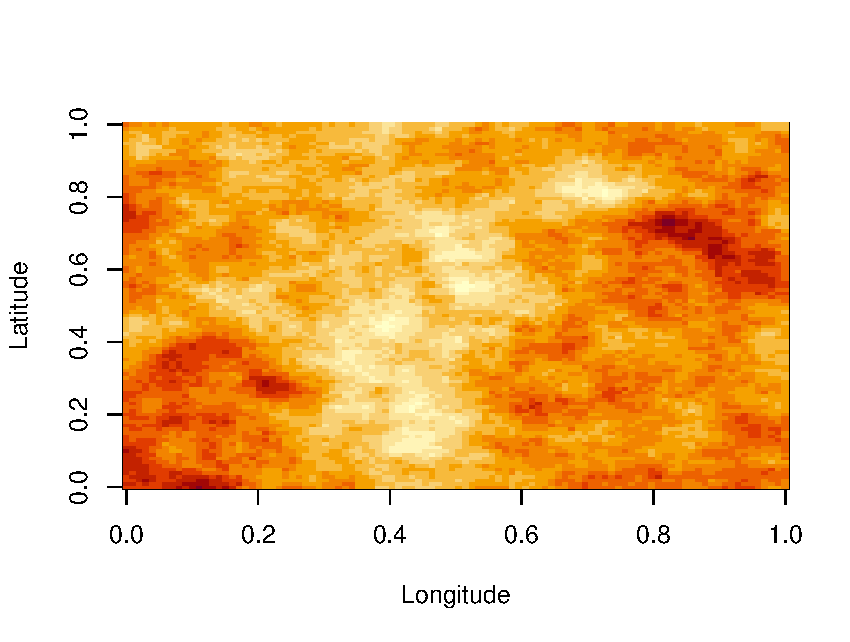
\includegraphics[width=
	\textwidth]{pics/GP_temp.pdf}
\end{figure}
\end{minipage}\begin{minipage}{8cm}
$\bs ullet$	Grid of $100^2$ points. \\[2mm]
$\bs ullet$ Fix the exponential kernel $\exp\{-\tfrac12\|\x-\x'\|\}$\\[2mm]
$\bs ullet$ Compute the $100^2\times 100^2$ covariance matrix\\[2mm]
$\bs ullet$ Get 1 sample from the corresponding distr.\\[2mm]
\end{minipage}
Handling a $10000$-dimensional Gaussian comes with its own computational challenges.  
\end{frame}

\begin{frame}{Spatial GP: Prediction}
\begin{enumerate}
    \item Combine training and test locations.
    \item Compute the covariance matrix using the kernel function.
    \item Use Gaussian conditioning formulas:
    \begin{align*}
        \mathbb{E}[\mathbf{y}_\text{test} | \mathbf{y}_\text{train}] &= \Sigma_\text{test,train}^\top \Sigma_\text{train,train}^{-1} \mathbf{y}_\text{train}, \\
        \text{Cov}(\mathbf{y}_\text{test} | \mathbf{y}_\text{train}) &= \Sigma_\text{test,test} - \Sigma_\text{test,train}^\top \Sigma_\text{train,train}^{-1} \Sigma_\text{test,train}.
    \end{align*}
\end{enumerate}
\end{frame}

\section{Nonparametric Regression with GPs}

\begin{frame}{Nonparametric Regression}
GPs can be used for nonparametric regression:
    \[
    y_i = f(\x_i) + \epsilon, \quad \eps_i \sim {N}(0, \sigma^2),\quad i=1,\ldots, n.
    \]
    
Prior over \( f:\R^d\to \R \): GP defined by \( m(\x) \) and \( k(\x, \x') \).
    \begin{itemize}
    \item In this sense GP defines a distribution over (random) functions $f: \R^d\to \R$.
    \end{itemize}    
    \medskip 
    
We have $f(\X)=(f(\x_1),\ldots,f(\x_n))\sim N_n(\nu,C)$ 
    \begin{itemize}
    \item $\nu_i=m(\x_i)$
    \item $C_{ij}=k(\x_i,\x_j)$
    \end{itemize}
    
    \begin{alertblock}{}
    	Say $d=1$. Given \( m(x) \) and \( k(x, x') \), how would you plot random samples of the corresponding random functions on $\R$?
    \end{alertblock}

\end{frame}

\begin{frame}{Nonparametric Regression}
	We have $\mathbf y\;=\;f(\mathbf{x})+\bs\eps$, and so $\y\sim N(m(\x),\Sigma+\sigma^2 I_n)$
   Prediction involves computing the posterior GP.
\end{frame}


%\begin{frame}{Code Example: Nonparametric Regression}
%\begin{minted}[frame=single,fontsize=\small]{r}
%# Generate training data
%x_train <- seq(0, 10, length.out = 10)
%y_train <- sin(x_train) + rnorm(length(x_train), sd = 0.1)
%
%# Test points
%x_test <- seq(0, 10, length.out = 100)
%
%# RBF kernel
%k <- function(x, x_prime, length_scale = 1) {
%    exp(-0.5 * (outer(x, x_prime, "-")^2) / length_scale^2)
%}
%
%# Covariance matrices
%K <- k(x_train, x_train)
%K_s <- k(x_train, x_test)
%K_ss <- k(x_test, x_test)
%
%# Posterior mean and covariance
%mu_s <- t(K_s) %*% solve(K) %*% y_train
%\end{minted}
%\end{frame}

\begin{frame}{Summary}
\begin{itemize}
    \item Gaussian Processes are a versatile tool for regression and spatial modeling.
    \item Key components:
    \begin{itemize}
        \item Mean function.
        \item Kernel function.
    \end{itemize}
    \item Next: Applications of GPs in high-dimensional data.
\end{itemize}
\end{frame}

\end{document}

